% Graphic for TeX using PGF
% Title: /home/isobel/Documents/McMaster/PythonCodes/DataAnalysis/Doc/Design/MG/UseHierarchy_IO.dia
% Creator: Dia v0.97.2
% CreationDate: Mon Nov  6 23:35:04 2017
% For: isobel
% \usepackage{tikz}
% The following commands are not supported in PSTricks at present
% We define them conditionally, so when they are implemented,
% this pgf file will use them.
\ifx\du\undefined
  \newlength{\du}
\fi
\setlength{\du}{15\unitlength}
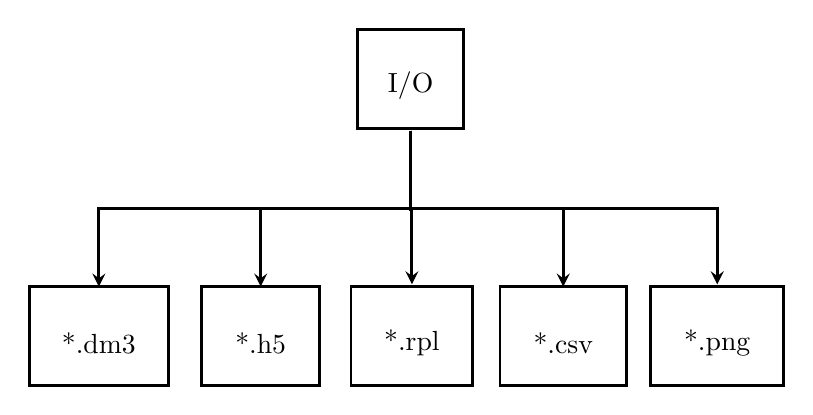
\begin{tikzpicture}
\pgftransformxscale{1.600000}
\pgftransformyscale{-1.600000}
\definecolor{dialinecolor}{rgb}{0.000000, 0.000000, 0.000000}
\pgfsetstrokecolor{dialinecolor}
\definecolor{dialinecolor}{rgb}{1.000000, 1.000000, 1.000000}
\pgfsetfillcolor{dialinecolor}
\definecolor{dialinecolor}{rgb}{1.000000, 1.000000, 1.000000}
\pgfsetfillcolor{dialinecolor}
\fill (23.517234\du,1.225277\du)--(23.517234\du,2.718610\du)--(25.114734\du,2.718610\du)--(25.114734\du,1.225277\du)--cycle;
\pgfsetlinewidth{0.070000\du}
\pgfsetdash{}{0pt}
\pgfsetdash{}{0pt}
\pgfsetmiterjoin
\definecolor{dialinecolor}{rgb}{0.000000, 0.000000, 0.000000}
\pgfsetstrokecolor{dialinecolor}
\draw (23.517234\du,1.225277\du)--(23.517234\du,2.718610\du)--(25.114734\du,2.718610\du)--(25.114734\du,1.225277\du)--cycle;
% setfont left to latex
\definecolor{dialinecolor}{rgb}{0.000000, 0.000000, 0.000000}
\pgfsetstrokecolor{dialinecolor}
\node at (24.315984\du,2.075277\du){I/O};
\definecolor{dialinecolor}{rgb}{1.000000, 1.000000, 1.000000}
\pgfsetfillcolor{dialinecolor}
\fill (18.571881\du,5.101413\du)--(18.571881\du,6.594746\du)--(20.671881\du,6.594746\du)--(20.671881\du,5.101413\du)--cycle;
\pgfsetlinewidth{0.070000\du}
\pgfsetdash{}{0pt}
\pgfsetdash{}{0pt}
\pgfsetmiterjoin
\definecolor{dialinecolor}{rgb}{0.000000, 0.000000, 0.000000}
\pgfsetstrokecolor{dialinecolor}
\draw (18.571881\du,5.101413\du)--(18.571881\du,6.594746\du)--(20.671881\du,6.594746\du)--(20.671881\du,5.101413\du)--cycle;
% setfont left to latex
\definecolor{dialinecolor}{rgb}{0.000000, 0.000000, 0.000000}
\pgfsetstrokecolor{dialinecolor}
\node at (19.621881\du,5.951413\du){*.dm3};
\definecolor{dialinecolor}{rgb}{1.000000, 1.000000, 1.000000}
\pgfsetfillcolor{dialinecolor}
\fill (21.168033\du,5.101413\du)--(21.168033\du,6.594746\du)--(22.948033\du,6.594746\du)--(22.948033\du,5.101413\du)--cycle;
\pgfsetlinewidth{0.070000\du}
\pgfsetdash{}{0pt}
\pgfsetdash{}{0pt}
\pgfsetmiterjoin
\definecolor{dialinecolor}{rgb}{0.000000, 0.000000, 0.000000}
\pgfsetstrokecolor{dialinecolor}
\draw (21.168033\du,5.101413\du)--(21.168033\du,6.594746\du)--(22.948033\du,6.594746\du)--(22.948033\du,5.101413\du)--cycle;
% setfont left to latex
\definecolor{dialinecolor}{rgb}{0.000000, 0.000000, 0.000000}
\pgfsetstrokecolor{dialinecolor}
\node at (22.058033\du,5.951413\du){*.h5};
\pgfsetlinewidth{0.070000\du}
\pgfsetdash{}{0pt}
\pgfsetdash{}{0pt}
\pgfsetmiterjoin
\pgfsetbuttcap
{
\definecolor{dialinecolor}{rgb}{0.000000, 0.000000, 0.000000}
\pgfsetfillcolor{dialinecolor}
% was here!!!
\pgfsetarrowsend{stealth}
{\pgfsetcornersarced{\pgfpoint{0.000000\du}{0.000000\du}}\definecolor{dialinecolor}{rgb}{0.000000, 0.000000, 0.000000}
\pgfsetstrokecolor{dialinecolor}
\draw (24.315984\du,2.753992\du)--(24.315984\du,3.927702\du)--(19.621881\du,3.927702\du)--(19.621881\du,5.101413\du);
}}
\pgfsetlinewidth{0.070000\du}
\pgfsetdash{}{0pt}
\pgfsetdash{}{0pt}
\pgfsetmiterjoin
\pgfsetbuttcap
{
\definecolor{dialinecolor}{rgb}{0.000000, 0.000000, 0.000000}
\pgfsetfillcolor{dialinecolor}
% was here!!!
\pgfsetarrowsend{stealth}
{\pgfsetcornersarced{\pgfpoint{0.000000\du}{0.000000\du}}\definecolor{dialinecolor}{rgb}{0.000000, 0.000000, 0.000000}
\pgfsetstrokecolor{dialinecolor}
\draw (24.315984\du,2.753992\du)--(24.315984\du,3.927702\du)--(22.058033\du,3.927702\du)--(22.058033\du,5.101413\du);
}}
% setfont left to latex
\definecolor{dialinecolor}{rgb}{0.000000, 0.000000, 0.000000}
\pgfsetstrokecolor{dialinecolor}
\node[anchor=west] at (24.315984\du,1.971944\du){};
% setfont left to latex
\definecolor{dialinecolor}{rgb}{0.000000, 0.000000, 0.000000}
\pgfsetstrokecolor{dialinecolor}
\node[anchor=west] at (19.621881\du,5.848080\du){};
\definecolor{dialinecolor}{rgb}{1.000000, 1.000000, 1.000000}
\pgfsetfillcolor{dialinecolor}
\fill (27.931710\du,5.101413\du)--(27.931710\du,6.594746\du)--(29.931710\du,6.594746\du)--(29.931710\du,5.101413\du)--cycle;
\pgfsetlinewidth{0.070000\du}
\pgfsetdash{}{0pt}
\pgfsetdash{}{0pt}
\pgfsetmiterjoin
\definecolor{dialinecolor}{rgb}{0.000000, 0.000000, 0.000000}
\pgfsetstrokecolor{dialinecolor}
\draw (27.931710\du,5.101413\du)--(27.931710\du,6.594746\du)--(29.931710\du,6.594746\du)--(29.931710\du,5.101413\du)--cycle;
% setfont left to latex
\definecolor{dialinecolor}{rgb}{0.000000, 0.000000, 0.000000}
\pgfsetstrokecolor{dialinecolor}
\node at (28.931710\du,5.951413\du){*.png};
\definecolor{dialinecolor}{rgb}{1.000000, 1.000000, 1.000000}
\pgfsetfillcolor{dialinecolor}
\fill (25.661463\du,5.101413\du)--(25.661463\du,6.594746\du)--(27.566463\du,6.594746\du)--(27.566463\du,5.101413\du)--cycle;
\pgfsetlinewidth{0.070000\du}
\pgfsetdash{}{0pt}
\pgfsetdash{}{0pt}
\pgfsetmiterjoin
\definecolor{dialinecolor}{rgb}{0.000000, 0.000000, 0.000000}
\pgfsetstrokecolor{dialinecolor}
\draw (25.661463\du,5.101413\du)--(25.661463\du,6.594746\du)--(27.566463\du,6.594746\du)--(27.566463\du,5.101413\du)--cycle;
% setfont left to latex
\definecolor{dialinecolor}{rgb}{0.000000, 0.000000, 0.000000}
\pgfsetstrokecolor{dialinecolor}
\node at (26.613963\du,5.951413\du){*.csv};
\definecolor{dialinecolor}{rgb}{1.000000, 1.000000, 1.000000}
\pgfsetfillcolor{dialinecolor}
\fill (23.417736\du,5.101413\du)--(23.417736\du,6.594746\du)--(25.252736\du,6.594746\du)--(25.252736\du,5.101413\du)--cycle;
\pgfsetlinewidth{0.070000\du}
\pgfsetdash{}{0pt}
\pgfsetdash{}{0pt}
\pgfsetmiterjoin
\definecolor{dialinecolor}{rgb}{0.000000, 0.000000, 0.000000}
\pgfsetstrokecolor{dialinecolor}
\draw (23.417736\du,5.101413\du)--(23.417736\du,6.594746\du)--(25.252736\du,6.594746\du)--(25.252736\du,5.101413\du)--cycle;
% setfont left to latex
\definecolor{dialinecolor}{rgb}{0.000000, 0.000000, 0.000000}
\pgfsetstrokecolor{dialinecolor}
\node at (24.335236\du,5.951413\du){*.rpl};
\pgfsetlinewidth{0.070000\du}
\pgfsetdash{}{0pt}
\pgfsetdash{}{0pt}
\pgfsetmiterjoin
\pgfsetbuttcap
{
\definecolor{dialinecolor}{rgb}{0.000000, 0.000000, 0.000000}
\pgfsetfillcolor{dialinecolor}
% was here!!!
\pgfsetarrowsend{stealth}
{\pgfsetcornersarced{\pgfpoint{0.000000\du}{0.000000\du}}\definecolor{dialinecolor}{rgb}{0.000000, 0.000000, 0.000000}
\pgfsetstrokecolor{dialinecolor}
\draw (24.315984\du,2.753417\du)--(24.315984\du,3.936900\du)--(24.335236\du,3.936900\du)--(24.335236\du,5.066997\du);
}}
\pgfsetlinewidth{0.070000\du}
\pgfsetdash{}{0pt}
\pgfsetdash{}{0pt}
\pgfsetmiterjoin
\pgfsetbuttcap
{
\definecolor{dialinecolor}{rgb}{0.000000, 0.000000, 0.000000}
\pgfsetfillcolor{dialinecolor}
% was here!!!
\pgfsetarrowsend{stealth}
{\pgfsetcornersarced{\pgfpoint{0.000000\du}{0.000000\du}}\definecolor{dialinecolor}{rgb}{0.000000, 0.000000, 0.000000}
\pgfsetstrokecolor{dialinecolor}
\draw (24.315984\du,2.753992\du)--(24.315984\du,3.927702\du)--(26.613963\du,3.927702\du)--(26.613963\du,5.101413\du);
}}
\pgfsetlinewidth{0.070000\du}
\pgfsetdash{}{0pt}
\pgfsetdash{}{0pt}
\pgfsetmiterjoin
\pgfsetbuttcap
{
\definecolor{dialinecolor}{rgb}{0.000000, 0.000000, 0.000000}
\pgfsetfillcolor{dialinecolor}
% was here!!!
\pgfsetarrowsend{stealth}
{\pgfsetcornersarced{\pgfpoint{0.000000\du}{0.000000\du}}\definecolor{dialinecolor}{rgb}{0.000000, 0.000000, 0.000000}
\pgfsetstrokecolor{dialinecolor}
\draw (24.315984\du,2.753993\du)--(24.315984\du,3.919223\du)--(28.931710\du,3.919223\du)--(28.931710\du,5.067307\du);
}}
\end{tikzpicture}
